The BRFSS 2015 dataset contains 328,135 training and 109,379 test observations, each with 321 inital features. The target variable, \texttt{\_MICHD}, reveals self-reported coronary heart disease or a myocardial infraction. Only $8.83\%$ of the training are positive, indicating a substantial class imbalance. Figure~\ref{fig:prevalence} highlights how positive rates vary across demographic and health-related factors, particularly age and general health.

\begin{figure}[h]
    \centering
    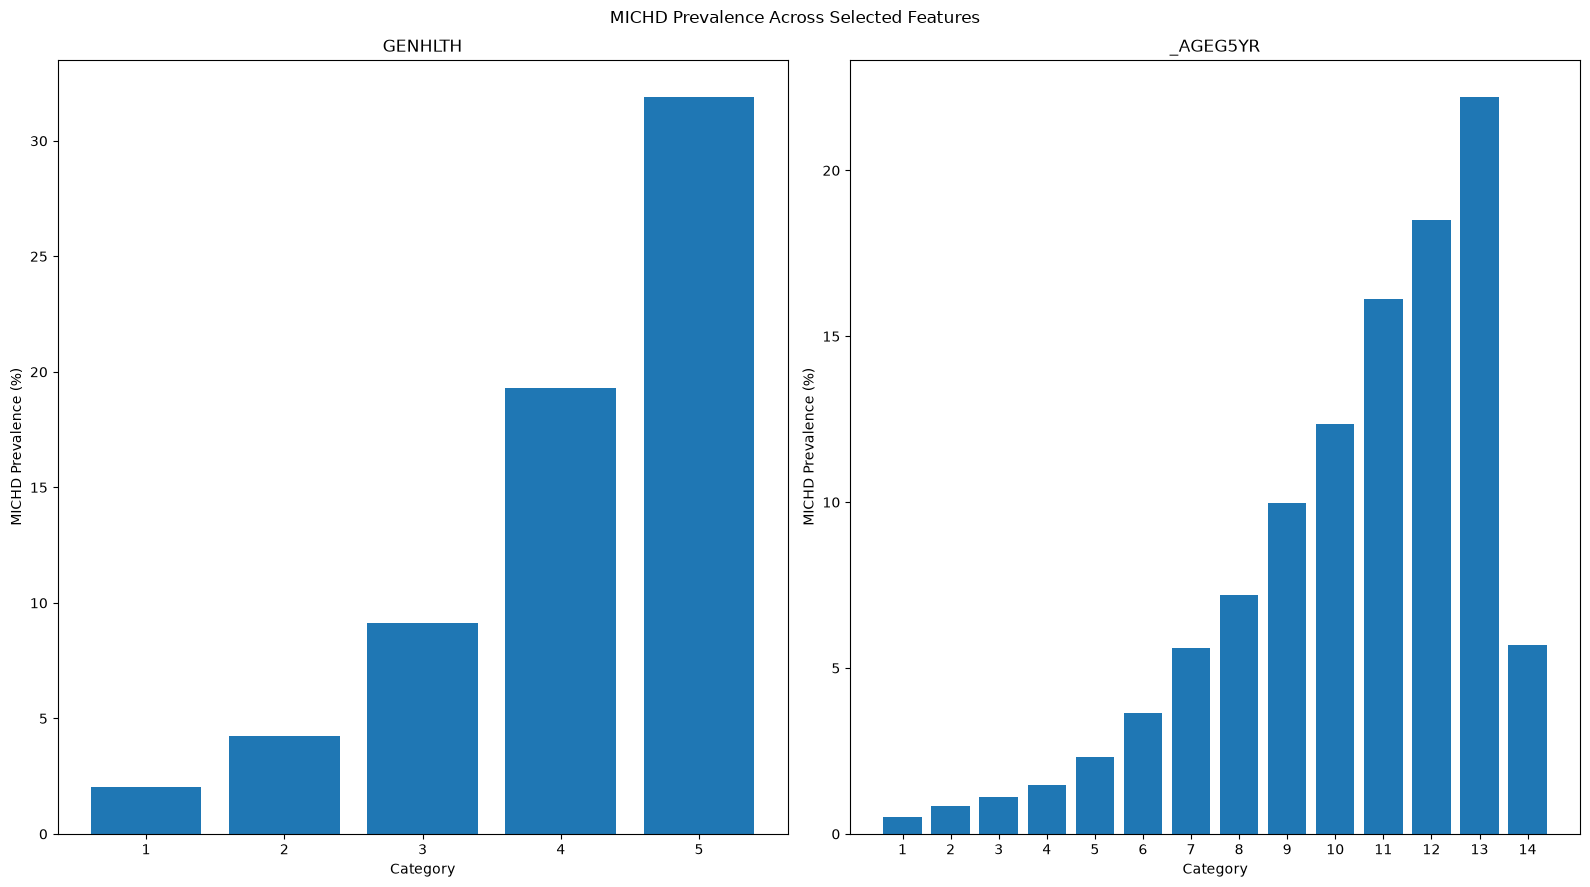
\includegraphics[width=0.45\linewidth]{figures/eda_michd_prevalence_2.png}
    \caption{Proportion of positive cases across age groups and general health categories}
    \label{fig:prevalence}
\end{figure}

Preprocessing involved removing administrative features and recoding special survey responses, as well as dropping constant features or those with over $90\%$ missing values. Remaining missing values were imputed using the median, followed by standardization. All transformations were fitted on training folds to prevent data leakage.